%*****************************************************************************************************             
%                       INSTITUT MINES-TELECOM, IMT Atlantique             
%                   Département Mathematical & Electrical Engineering           
%                                Technopôle de Brest-Iroise                   
%                                 CS 83818 - 29238 BREST Cedex 3                                                       
%                                     **  Tous droits réservés **                                     
%
% NOM DU PROJET : Document de cadrage - Projet S7 2026-2027 (IMT Atlantique)
%***********************************************************************************************

\documentclass[11pt,a4paper,french]{article}

\usepackage{babel}
\usepackage[utf8]{inputenc}
\usepackage[T1]{fontenc}

\usepackage{newtxtext} % Police pour texte
\usepackage{newtxmath} % Police pour formules
\usepackage{textcomp}
\usepackage{graphicx}
\usepackage{amsmath}
\usepackage{microtype}

\usepackage{framed}   % Permet de surligner les résultats importants
\usepackage{tabularx} % Tableaux du document de cadrage
\usepackage{array}
\usepackage{enumitem}
\usepackage{eurosym}
\usepackage{float}
% \newcommand{\sectionbreak}{\clearpage} % désactivé : faisait dépasser la limite de 15 pages

% L'option "copyright" affiche la licence Creative Common en 4eme de couverture
\usepackage[copyright]{../sty/imta} 
\usepackage{tikz}     % Diagrammes (contexte, pieuvre, organigramme des lots)
\usetikzlibrary{positioning,calc,fit,shapes.geometric}
\usepackage{pgfgantt} % Diagramme de Gantt
\usepackage{colortbl}  % Cellules colorées (tableau des risques)
% Couleurs communes aux schémas
\definecolor{lotA}{HTML}{2E75B6}% intégration du bateau
\definecolor{lotB}{HTML}{3A9D5D}% vision embarquée
\definecolor{lotC}{HTML}{C0504D}% intégration vision et bateau
\definecolor{lotD}{HTML}{7F7F7F}% gestion de projet
\definecolor{critiqueHigh}{RGB}{250,190,190}% criticité élevée
\definecolor{critiqueMed}{RGB}{255,235,175}% criticité moyenne
\definecolor{critiqueLow}{RGB}{210,245,215}% criticité faible

% Signets et hyperliens (à charger en dernier)
\usepackage[colorlinks=true,linkcolor=black,urlcolor=blue,citecolor=IMTAbleu]{hyperref}
% Mise en évidence de textes par icônes et barre verticale
\usepackage{../sty/awesomebox}

%----------------- Métadonnées du PDF ---------------------------------------------------------
\hypersetup{
    pdfinfo = {
        Author = {Reda El Mekkaoui; Adam-Sabri Hlaoua; Guillaume Leroy; Ewen Gourmelen; Selma Ben-Abdelkader; Rana Brini},
        Title = {Intégration d'une plateforme USV et d'une chaîne de détection temps réel assistée par intelligence artificielle pour l'aide à la navigation autonome},
        Keywords = {USV; Intelligence Artificielle; Navigation autonome; Cerema}
    }
}

%--------------------------- Définition du contenu du pied de page ----------------------------
\IMTAfooter{\thereportnumber}

%-------------------- Informations de copyright pour quatrième de couverture ------------------
\IMTCopyright{[Choisir une licence Creative Commons\\\URLcclicence\\
             et l’apposer ici à la place de cette phrase en enlevant les crochets]}

%----------------- Définitions d'ensembles et d'opérateurs mathématiques ----------------------
\def\Cset{\mathbb{C}} % complexes
\def\Hset{\mathbb{H}} % hilbert
\def\Nset{\mathbb{N}} % entiers naturels
\def\Qset{\mathbb{Q}} % rationnels
\def\Rset{\mathbb{R}} % reels
\def\Zset{\mathbb{Z}} % entiers relatifs
\def\Dset{\mathbb{D}} % disque unite ouvert
\def\Eset{\mathbb{E}} % esperance mathematique

%---------------------- Commandes du document de cadrage --------------------------------------
\newif\ifconsignes
\consignesfalse
\newcommand{\consigne}[1]{\ifconsignes{\color{gray}\itshape #1\par}\fi}

\providecommand{\todo}[1]{\textcolor{red}{[\textbf{À compléter :} #1]}}

\newcolumntype{L}{>{\raggedright\arraybackslash}X}
% Flèche de dépendance fin -> début entre deux barres nommées du Gantt.
% L'argument optionnel est la hauteur du segment horizontal au-dessus de la barre d'arrivée
% (0.275cm = un demi-rang pour des barres sur des rangs voisins).
\newcommand{\ganttdep}[3][0.275cm]{%
  \draw[-latex, thick, gray!70!black, rounded corners=1pt]
    (#2.east) -- ++(0.18cm,0) |- ([xshift=-0.18cm, yshift=#1]#3.west) |- (#3.west);}
\addto\captionsfrench{\renewcommand{\tablename}{Tableau}}

%-------------------------------------- FIN DES DEFINITIONS ----------------------------------

\begin{document}

%---------------------------------------------------------------------------------------------
%                                   PAGE DE TITRE
%---------------------------------------------------------------------------------------------

\entity{
    \textbf{\large{IMT Atlantique}}\\
    Projet Commande Entreprise\\
    S7 2026-2027 \\
    Campus de Brest
}

\MentionSpeciale{\textbf{\Large Document de synthèse -- Projet numéro 20}}
\title{Intégration d'une plateforme USV et d'une chaîne de détection temps réel assistée par intelligence artificielle pour l'aide à la navigation autonome.}

\author{\vspace{1cm}\textit{%
    Reda El Mekkaoui \and
    Adam-Sabri Hlaoua \and
    Guillaume Leroy \and
    Ewen Gourmelen \and
    Selma Ben-Abdelkader \and
    Rana Brini%
}%
}

\contributors{%
    \vspace{0.4cm}% Petit espace vertical pour aérer sous les auteurs
    \begin{flushleft}
        Encadré par : \textit{Matthieu Arzel} (IMT Atlantique) \\
        Clients : \textit{Antoine Douchin} (Cerema) \\
        Destinataires : Antoine Douchin (Cerema), Matthieu Arzel (IMT Atlantique)
    \end{flushleft}%
}

\version{2}

\maketitle

% --- HISTORIQUE DES RÉVISIONS ---
\begin{table}[h]
    \centering
    \caption*{\large \textbf{Historique des révisions du document}}
    \small
    \begin{tabularx}{\textwidth}{@{}ccp{2.2cm}Lp{2.8cm}@{}}
        \toprule
        \textbf{Version} & \textbf{Révision} & \textbf{Date} & \textbf{Description des changements} & \textbf{Auteur} \\
        \midrule
        1 & 0 & 02/10/2026 & Version initiale, envoyée au client et au tuteur école & Tout le groupe \\
        2 & 0 & 04/10/2026 & Prise en compte de la réunion du 02/10/2026 : scénario d'usage cible, fonction FS2, pilotage par gouverne, périmètre, réunions client toutes les deux semaines & Tout le groupe \\
        \bottomrule
    \end{tabularx}
\end{table}

% --- RELECTEURS ---
\begin{table}[h]
    \centering
    \caption*{\large \textbf{Rédacteur et relecteur par partie}}
    \small
    Chaque partie a un rédacteur référent, à contacter pour toute question sur son contenu.\par\vspace{0.2cm}
    \begin{tabularx}{\textwidth}{@{}Lp{3.4cm}p{4.6cm}@{}}
        \toprule
        \textbf{Partie du document} & \textbf{Rédacteur référent} & \textbf{Contact} \\
        \midrule
        Page de garde, introduction, présentation du projet (section~\ref{sec:presentation}) & Reda El Mekkaoui & reda.el-mekkaoui@imt-atlantique.net \\
        Cahier des charges fonctionnel (section~\ref{sec:cdcf}) & Ewen Gourmelen & ewen.gourmelen@imt-atlantique.net \\
        Plan de travail (section~\ref{sec:plan-travail}) & Rana Brini & rana.brini@imt-atlantique.net \\
        Organisation : équipe, parties prenantes, lots, planification, communication (section~\ref{sec:organisation}) & Guillaume Leroy & guillaume.leroy@imt-atlantique.net \\
        Organisation : analyse des risques (section~\ref{sec:risques}) & Adam-Sabri Hlaoua & adam-sabri.hlaoua@imt-atlantique.net \\
        Validation du projet et conclusion (sections~\ref{sec:validation-projet} et~\ref{sec:conclusion}) & Selma Ben-Abdelkader & selma.ben-abdelkader@imt-atlantique.net \\
        Références bibliographiques et annexes & Tout le groupe & -- \\
        \bottomrule
    \end{tabularx}
\end{table}

\newpage

%% Affichage des listes et tables.
\IMTAsommaire
\newpage
%\IMTAlistefigures  % commenter pour ne pas avoir la liste des figures (absente du modèle de cadrage)
%\IMTAlistetableaux   % commenter pour ne pas avoir la liste des tables (absente du modèle de cadrage)
%---------------------------------------------------------------------------------------------
%                 CORPS DU DOCUMENT : ordre de la consigne du document de synthèse
%---------------------------------------------------------------------------------------------



\section{Introduction}

Ce document fait le point sur le lancement du projet : ce que l'équipe a compris du besoin du Cerema, ce qu'elle va réaliser et comment elle s'organise. Il s'adresse au client et au tuteur école, prépare la revue de projet et sert à affiner le besoin avec le client. Il s'appuie sur la fiche du sujet, les travaux du projet 2025, la réunion de lancement et les échanges avec le Cerema (section~\ref{sec:bibliographie}). Le tableau~\ref{tab:terminologie} définit les termes techniques utilisés.

\begin{table}[H]
\centering
\small
\caption{Terminologie}
\label{tab:terminologie}
\begin{tabularx}{\textwidth}{@{}>{\raggedright\arraybackslash}p{3.8cm}L@{}}
\toprule
\textbf{Terme} & \textbf{Définition} \\
\midrule
USV (\emph{Unmanned Surface Vehicle}) & Drone de surface : bateau sans équipage, télépiloté ou autonome. \\
PCE & Projet Commande Entreprise, réalisé par des élèves pour un partenaire extérieur. \\
Autopilote (Pixhawk, ArduPilot) & Carte et logiciel qui commandent les moteurs et gèrent la navigation. \\
Station sol (QGroundControl) & Ordinateur qui permet de piloter le bateau, de programmer et de suivre les missions. \\
Ordinateur compagnon & Ordinateur embarqué (ici un Raspberry Pi 4) qui analyse les images et dialogue avec l'autopilote. \\
MAVLink & Langage de communication entre l'autopilote, l'ordinateur compagnon et la station sol. \\
Point de passage (\emph{waypoint}) & Position que le bateau doit rejoindre lors d'une mission programmée. \\
ESC & Variateur qui commande la vitesse d'un moteur. \\
YOLO & Famille de modèles d'IA qui détectent des objets dans une image. \\
Métadonnées de détection & Résultats du modèle (cadre, classe, score de confiance) transmis avec l'image, exploitables par l'ordinateur compagnon. \\
OCR & Reconnaissance de caractères, ici pour lire l'immatriculation d'un navire. \\
AIS & Système par lequel un navire émet en continu son identité, sa position et sa vitesse. \\
Gouverne & Surface orientable qui dirige le bateau, ici commandée par un moteur. \\
\bottomrule
\end{tabularx}
\end{table}

\section{Présentation du projet}
\label{sec:presentation}

% ---------------------------------------------------------------------------
\subsection{Contexte}
\label{sec:contexte-projet}

\paragraph{Le client et son besoin.}
Le Cerema est un établissement public qui accompagne l'État et les collectivités, notamment dans la gestion des risques, et qui utilise des drones pour collecter des données sur le terrain. Sa direction Risques, Eaux et Mer veut mieux surveiller les zones maritimes où la navigation, le mouillage ou la pêche sont interdits ou limités, avec une solution à bas coût qui aide les contrôleurs en mer. Le drone doit détecter et identifier les navires présents dans ces zones.

\paragraph{L'existant : le projet 2025.}
Ce projet prolonge le PCE 2025 « Conception d'un micro drone de surface », résumé dans le tableau~\ref{tab:acquis-2025}. Sa principale limite : chaque partie a été testée en laboratoire, mais jamais l'ensemble en conditions réelles. En vision, l'équipe 2025 a proposé de détecter en basse résolution, qui consomme environ 23~\% de moins, puis de confirmer en haute résolution avec la caméra IA.

\begin{table}[H]
\centering
\small
\caption{Acquis du projet 2025}
\label{tab:acquis-2025}
\begin{tabularx}{\textwidth}{@{}p{2.4cm}LL@{}}
\toprule
\textbf{Partie} & \textbf{Réalisé} & \textbf{Reste ouvert} \\
\midrule
Énergie & Batteries et panneaux solaires dimensionnés sur la baie de Saint-Brieuc (coût estimé à 2495,4~\euro{}). & Calculs à affiner. \\
Coque & Catamaran modélisé ; maquette au 1/3 testée en bassin. & Pas de coque à l'échelle 1. \\
Électronique & Composants choisis ; un moteur piloté par le Pixhawk ; arrêt des moteurs sur perte de signal validé ; GPS relié au Pixhawk. & Ensemble jamais testé en conditions réelles. \\
Vision & Modèle YOLO entraîné sur environ 7000 images de 6 types de navires ; au moins 90~\% de détection sur des images dégradées (gouttes, flou). & Collecter des images réelles pour réentraîner le modèle. \\
\bottomrule
\end{tabularx}
\end{table}

\paragraph{Ce qui existe ailleurs.}
Des drones de surface existent déjà, par exemple le Bathydrone NANO (Escadrone), le projet PLANCHA (Ifremer) ou le WiBoat C3 (ADCPro). La plupart servent à l'observation et non au contrôle : leur autonomie est faible et leurs contraintes de stabilité sont différentes. La forme en catamaran revient souvent pour sa stabilité.

% ---------------------------------------------------------------------------
\subsection{Enjeux et problématique}

\begin{itemize}
  \item \textbf{Pour le client :} disposer d'un outil de surveillance maritime à bas coût, capable d'être autonome pendant une longue durée, au service des politiques publiques de gestion des risques côtiers.
  \item \textbf{Pour le projet :} faire évoluer le drone de 2025 vers une plateforme qui fonctionne, testée en conditions réelles, sur laquelle ajouter progressivement de l'autonomie. Il ne s'agit ni d'une réponse à la concurrence ni d'une recherche scientifique, mais de l'évolution d'un produit existant.
\end{itemize}

\noindent\textbf{Problématique :} comment concevoir et intégrer un drone de surface autonome, robuste aux conditions marines et de moins d'un mètre, capable d'identifier les infractions grâce à l'IA, tout en respectant de fortes contraintes d'autonomie énergétique et de puissance de calcul embarquée ?

% ---------------------------------------------------------------------------
\subsection{Finalité, mission, objectifs}
\label{sec:finalite-mission-objectifs}

\paragraph{Finalité.} Aider le Cerema à développer un drone de surface pour surveiller les zones maritimes réglementées, capable de détecter et d'identifier les navires.

\paragraph{Mission.} Obtenir un bateau qui fonctionne, pilotable à distance, servant de base pour ajouter progressivement de l'autonomie. La fiche du sujet prévoit trois étapes : piloter le bateau depuis un ordinateur grâce à un autopilote, ajouter un ordinateur embarqué qui dialogue avec l'autopilote, puis ajouter une brique d'IA qui détecte les navires et déclenche des alertes. Les attentes sont :
\begin{itemize}
  \item \textbf{bateau :} assembler durablement les composants, rendre le bateau capable de suivre une mission programmée par points de passage, repérer les composants manquants (modem…) et choisir la motorisation ;
  \item \textbf{IA :} détecter les navires, puis reconnaître leur type, lire leur immatriculation et suivre leur activité ; rendre la détection fiable par mauvais temps (pluie, roulis) ; faire fonctionner deux caméras sur un Raspberry Pi 4. Elle doit aussi consommer le moins possible.
\end{itemize}

\paragraph{Objectifs.}
\begin{enumerate}
  \item \textbf{Un cahier des charges complet du produit}, précisé au fil du projet (fin octobre).
  \item \textbf{Un prototype qui navigue} : pilotable à distance, capable de suivre une mission programmée, de tenir un cap et de s'arrêter (fin novembre).
  \item \textbf{Une détection de navires qui fonctionne sur Raspberry Pi 4}, y compris par mauvais temps, avec au moins 90~\% de détection (fin novembre) ; si possible, reconnaître le type de navire, son immatriculation et son activité.
  \item \textbf{L'intégration de la vision au bateau}, étanche et qui consomme le moins possible.
  \\
\end{enumerate}

% ---------------------------------------------------------------------------
\subsection{Périmètre}
\label{sec:perimetre}

À la demande du client, l'équipe se concentre sur deux parties : l'assemblage du bateau et la vision embarquée (figure~\ref{fig:perimetre}). La coque et le bilan énergétique, traités en 2025, sont hors périmètre. Les essais se font sur un catamaran bricolé de plus d'un mètre fourni par le Cerema ; le produit final visé fera moins d'un mètre.

\begin{figure}[H]
\centering
\resizebox{\textwidth}{!}{%
\begin{tikzpicture}[font=\small,
  zone/.style={draw, rounded corners, thick, align=left, text width=4.6cm, inner sep=6pt, minimum height=3.6cm, anchor=north}]
  \node[zone, draw=lotB, fill=lotB!10] (dans) at (0,0) {\textbf{Dans le périmètre}\\[3pt]
    \textbullet~Assemblage durable des composants\\
    \textbullet~Choix de la motorisation\\
    \textbullet~Missions par points de passage\\
    \textbullet~Détection de navires sur Raspberry Pi 4\\
    \textbullet~Détection par mauvais temps\\
    \textbullet~Cahiers des charges précis};
  \node[zone, draw=orange!80!black, fill=orange!10] (opt) at (5.4,0) {\textbf{Si le temps le permet}\\[3pt]
    \textbullet~Reconnaître le type de navire\\
    \textbullet~Lire son immatriculation\\
    \textbullet~Suivre son activité\\
    \textbullet~S'approcher du navire pour l'identifier};
  \node[zone, draw=lotC, fill=lotC!10] (hors) at (10.8,0) {\textbf{Hors périmètre}\\[3pt]
    \textbullet~Conception de la coque\\
    \textbullet~Bilan énergétique et panneaux solaires\\
    \textbullet~Fabrication du produit final de moins d'un mètre\\
    \textbullet~Conception de la gouverne\\
    \textbullet~Caméra 360°};
\end{tikzpicture}}
\caption{Périmètre du projet}
\label{fig:perimetre}
\end{figure}

\section{Cahier des charges fonctionnel}
\label{sec:cdcf}

% ---------------------------------------------------------------------------
\subsection{Contexte d'utilisation du système}
\label{sec:contexte}

Au service du Cerema et des autorités maritimes, le drone surveille en continu les zones réglementées. En détectant et en identifiant systématiquement les navires en infraction, il optimise l'efficacité de la surveillance maritime et contribue directement à restreindre les activités de pêche non autorisées.
\\
La figure~\ref{fig:bete-cornes} résume le besoin :

\begin{figure}[H]
\centering
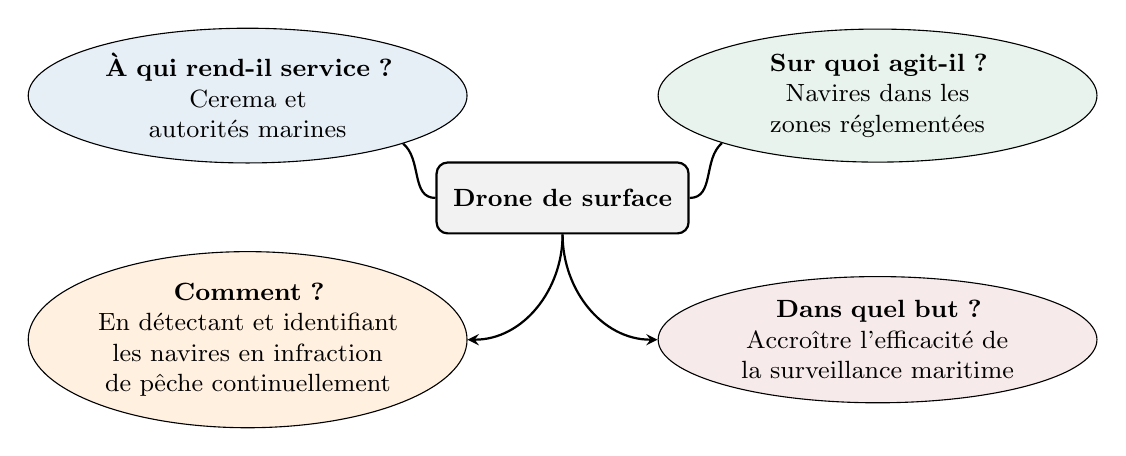
\begin{tikzpicture}[font=\small,
  bulle/.style={draw, ellipse, align=center, inner sep=2pt}]
  \node[bulle, fill=lotA!12, text width=3.8cm] (qui) at (-4,1.6) {\textbf{À qui rend-il service ?}\\ Cerema et autorités marines};
  \node[bulle, fill=lotB!12, text width=3.8cm] (quoi) at (4,1.6) {\textbf{Sur quoi agit-il ?}\\ Navires dans les zones réglementées};
  \node[draw, thick, rounded corners, fill=gray!10, minimum width=3.2cm, minimum height=0.9cm] (usv) at (0,0.3) {\textbf{Drone de surface}};
  \node[bulle, fill=orange!12, text width=3.8cm] (comment) at (-4,-1.5) {\textbf{Comment ?}\\ En détectant et identifiant les navires en infraction de pêche continuellement};
  \node[bulle, fill=lotC!12, text width=3.8cm] (but) at (4,-1.5) {\textbf{Dans quel but ?}\\ Accroître l'efficacité de la surveillance maritime};
  \draw[thick] (qui.south east) to[out=-40, in=180] (usv.west);
  \draw[thick] (usv.east) to[out=0, in=220] (quoi.south west);
  \draw[->, >=stealth, thick] (usv.south) to[out=-90, in=0] (comment.east);
  \draw[->, >=stealth, thick] (usv.south) to[out=-90, in=180] (but.west);
\end{tikzpicture}
\caption{Expression du besoin}
\label{fig:bete-cornes}
\end{figure}


Ce drone de surface navigue de manière autonome en suivant un parcours GPS préalablement programmé par les opérateurs. Pour maintenir son cap, il ajuste et corrige sa trajectoire par lui-même tout au long de la mission. Conçu pour opérer de manière ininterrompue, il doit disposer d'une forte autonomie. Sa mission principale consiste à repérer et identifier formellement les navires pratiquant la pêche illicite. Dès qu'une infraction est constatée, le drone transmet une alerte immédiate aux équipes, leur fournissant la position et l'identité du bateau suspect.



\begin{figure}[H]
\centering
\resizebox{\textwidth}{!}{%
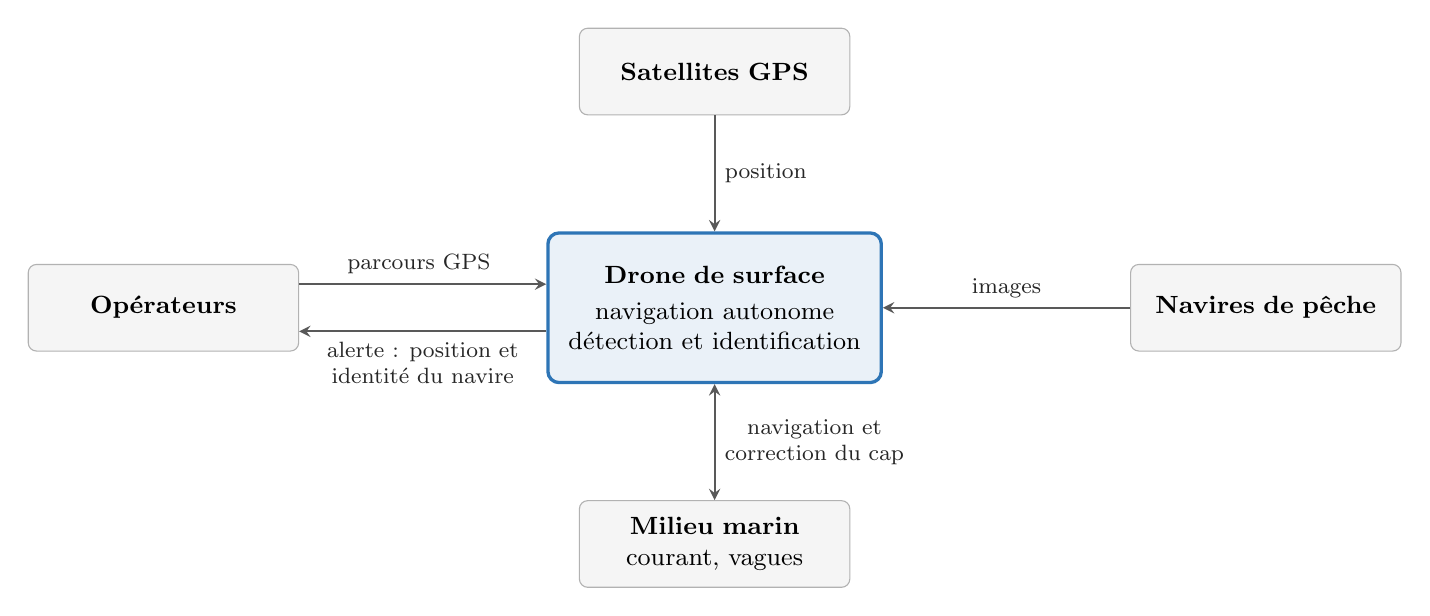
\begin{tikzpicture}[font=\small,
  ext/.style={draw=gray!60, rounded corners=3pt, fill=gray!8, align=center, text width=3.2cm, minimum height=1.1cm},
  fl/.style={->, >=stealth, thick, draw=gray!70!black},
  et/.style={font=\footnotesize, align=center, text=gray!30!black}]
  \node[draw=lotA, very thick, rounded corners=4pt, fill=lotA!10, align=center, text width=4cm, minimum height=1.9cm] (usv) at (0,0)
    {\textbf{Drone de surface}\\[2pt] navigation autonome\\ détection et identification};
  \node[ext] (op)  at (-7,0)  {\textbf{Opérateurs}};
  \node[ext] (nav) at (7,0)   {\textbf{Navires de pêche}};
  \node[ext] (sat) at (0,3)   {\textbf{Satellites GPS}};
  \node[ext] (mer) at (0,-3)  {\textbf{Milieu marin}\\ courant, vagues};
  \draw[fl] ([yshift=3mm]op.east) -- node[et, above]{parcours GPS } ([yshift=3mm]usv.west);
  \draw[fl] ([yshift=-3mm]usv.west) -- node[et, below]{alerte : position et\\ identité du navire} ([yshift=-3mm]op.east);
  \draw[fl] (nav) -- node[et, above]{images} (usv);
  \draw[fl] (sat) -- node[et, right]{position} (usv);
  \draw[fl, <->] (usv) -- node[et, right]{navigation et\\ correction du cap} (mer);
 \end{tikzpicture}}
\caption{Diagramme de contexte : le drone et les éléments extérieurs avec lesquels il interagit}
\label{fig:contexte}
\end{figure}

% ---------------------------------------------------------------------------
\subsection{Expression fonctionnelle du besoin}

\subsubsection{Fonctions de service et de contrainte}
Avant de détailler les fonctions du système, il convient de distinguer l'objectif final visé par le Cerema des objectifs réalisables dans le cadre de ce Projet Commande Entreprise (PCE). Si le produit final ambitionne d'être un navire totalement autonome sur un an, capable d'identifier formellement les actions de pêche illicite, notre projet n'a pas pour vocation de livrer ce produit fini.



L'objectif de notre équipe est de réaliser une preuve de concept (PoC) fonctionnelle en se concentrant sur deux verrous technologiques majeurs :

\begin{enumerate}
    \item L'intégration matérielle et logicielle sur le navire : l'assemblage des composants pour permettre le pilotage à distance, l'exécution d'une mission de patrouille et l'interaction avec un opérateur. 
    \item La détection par intelligence artificielle : le développement et l'intégration d'un modèle de vision (YOLO) embarqué, capable de détecter et d'identifier les navires présents dans une zone.
\end{enumerate}

Par conséquent, les critères et niveaux d'exigence présentés dans le tableau fonctionnel ci-dessous (Tableau ~\ref{tab:fonctions}) traduisent les objectifs de notre projet technique à l'horizon de décembre 2026, et non les spécifications du drone final.










\begin{table}[H]
\centering
\small
\caption{Fonctions du système, avec leurs critères de valeur, niveaux, flexibilité et priorité. FP : fonction principale, FS : fonction secondaire, FC : fonction de contrainte.}
\label{tab:fonctions}
\begin{tabularx}{\textwidth}{@{}Lp{3cm}p{2.4cm}p{1.8cm}p{1.3cm}@{}}
\toprule
\textbf{Fonction} & \textbf{Critère(s)} & \textbf{Niveau(x)} & \textbf{Flexibilité} & \textbf{Priorité} \\
\midrule
FP1 -- Être piloté manuellement avec un système de propulsion fixe couplée avec des gouvernes & réactivité de la commande & réponse < 1 s & Moyenne & 1 \\
\addlinespace
FP2 -- Détecter à bord, en temps réel, les navires présents dans la zone, y compris par pluie, roulis ou mouvement & Taux de détection ; cadence d'analyse & Taux $\geq$ 90 \% ; au moins 1 image analysée toutes les 5 s (niveaux atteints ou envisagés en 2025) & Moyenne & 1 \\
\addlinespace
FP3 -- Transmettre à l'opérateur l'état de la mission en temps réel (position, état du système) & Fréquence de mise à jour & Au moins 1 mise à jour par minute & Forte & 1 \\
\addlinespace
FP4 -- Générer une alerte à destination de l'opérateur lors d'une détection & Délai d'alerte & $\leq$ 5 s après la détection & Moyenne & 2 \\
\addlinespace

FP5 -- Suivre de façon autonome un cap, pouvoir suivre une trace GPS définie par points de passage & Précision du suivi de trajectoire & Écart $\leq$ 5 m à chaque point de passage & Moyenne & 2 \\
\addlinespace

FS1 -- Déterminer la catégorie, l'immatriculation et l'activité d'un navire détecté & Part des navires correctement identifiés & À définir avec le Cerema & Forte & 3 \\
\addlinespace

FS2 -- Modifier et optimiser la trajectoire du drône de surface pour s'approcher du bateau suspect pour une meilleure identification & Précision du suivi de trajectoire & Écart maximal de ± 5 mètres par rapport à la trajectoire calculée & Forte & 3 \\
\addlinespace

FC1 -- Utiliser le matériel mis à disposition (tableau~\ref{tab:materiel}) & Conformité à la liste du matériel & Matériel du tableau~\ref{tab:materiel} & Faible & 1 \\
\addlinespace
FC2 -- Communiquer entre l'ordinateur compagnon et l'autopilote par le protocole MAVLink & Protocole utilisé & MAVLink & Nulle & 1 \\
\addlinespace
FC3 -- Limiter la consommation energétique & Durée de fonctionnement & Au moins 1h d'essai en continu & Moyenne & 2 \\
\addlinespace
FC4 -- Respecter les contraintes de sécurité & Comportement sur perte de liaison & Arrêt des moteurs (fonction validée en 2025) & Nulle & 1 \\
\bottomrule
\end{tabularx}
\end{table}

\subsubsection{Scénarios}
\label{sec:scenarios}

\paragraph{Scénario nominal.} 
\begin{enumerate}
  \item l'opérateur lance une patrouille depuis la station sol (FP5) ;
  \item le bateau parcourt la zone seul et envoie son état (FP5, FP3) ;
  \item la caméra détecte un navire (FP2) ;
  \item l'opérateur reçoit une alerte (FP4) ;
  \item l'opérateur peut prendre la main sur le pilotage (FP1).
\end{enumerate}

\paragraph{Scénario d'usage cible.} Issu de la réunion du 02/10/2026 avec le Cerema, il prolonge le scénario nominal en couplant la vision et la navigation. Pour économiser l'énergie du Raspberry Pi, l'analyse est répartie entre plusieurs petits modèles spécialisés, appelés experts, qui ne tournent jamais tous en même temps. Les étapes 1, 2, 5 et 6 en forment le socle ; les étapes 3 et 4 (FS1, FS2) seront réalisées si le temps le permet.
\begin{enumerate}
  \item le bateau patrouille seul sur une route programmée et envoie son état à l'opérateur (FP5, FP3) ;
  \item un modèle léger surveille en permanence ; quand un navire est détecté sur plusieurs images consécutives, le seuil d'alerte est franchi (FP2) ;
  \item un petit modèle de décision réveille l'expert utile : catégorie du navire, lecture de l'immatriculation, trajectoire d'approche (liste non exhaustive) (FS1) ;
  \item l'ordinateur compagnon transmet à l'autopilote une consigne de navigation issue de cette analyse : le bateau quitte sa route, se dirige vers le navire et le contourne, sans contact, jusqu'à ce que l'immatriculation soit lisible (FS2, FC2) ;
  \item l'opérateur reçoit une alerte courte, sans image : position, catégorie, immatriculation (FP4) ;
  \item le bateau reprend sa patrouille ; l'opérateur peut reprendre la main à tout moment (FP5, FP1).
\end{enumerate}

\paragraph{Cas limites.} 
\begin{itemize}
  \item perte de la liaison : arrêt des moteurs (fonction déjà validée en 2025) ;
  \item perte du GPS : arrêt et alerte à l'opérateur ;
  \item batterie faible : alerte à l'opérateur ;
  \item détection douteuse : image transmise à l'opérateur, qui confirme.
  \\
\end{itemize}

% ---------------------------------------------------------------------------
\subsection{Validation du besoin}
\label{sec:validation-besoin}

Chaque fonction sera d'abord testée seule, composant par composant, puis avec les autres. La fiche prévoit des essais de navigation manuelle et automatique (FP1, FP5), des tests de détection de bateau en action de pêche (FP2), des tests de communication entre l'opérateur et le drone de surface (FP3,FP4) et la vérification des missions automatiques (FP5). L'équipe y ajoute des tests de détection sur des images réelles et dégradées (FP2). Les méthodes, seuils et responsables sont détaillés en section~\ref{sec:validation-projet}.
\\

\section{Le plan de travail}
\label{sec:plan-travail}

% ---------------------------------------------------------------------------
\subsection{Méthodologie}

L'équipe suit une méthode hybride. L'ensemble du projet suit un cycle en V : cahiers des charges, conception, intégration, tests, puis recette. À l'intérieur de chaque lot, elle travaille de façon agile, par itérations de deux semaines rythmées par les réunions avec le client (figure~\ref{fig:gantt}) et par un point d'équipe hebdomadaire. Cela permet d'ajuster le travail au fil de la découverte du matériel. Dans un premier temps, l'équipe va se diviser en deux groupes selon les compétences afin de réaliser les premières grosses tâches en parallèle puis leur intégration.

% ---------------------------------------------------------------------------
\subsection{Étapes du projet}

Les deux parties avancent en parallèle, chacune confiée à un groupe de trois, puis sont réunies. Chaque groupe rédige un cahier des charges précis une fois le matériel pris en main ; il évoluera au cours du projet.
\\
\paragraph{Intégration du bateau.}
\begin{enumerate}
  \item \textbf{Prise en main :} comprendre les composants, vérifier le schéma d'assemblage et repérer ce qui manque, faire tourner les moteurs et piloter le bateau.
  \item \textbf{Cahier des charges précis} de la partie matérielle.
  \item \textbf{Choix du type de moteur et de gouvernail} : choisir entre les différents moteurs ainsi que le système de manoeuvre.
  \item \textbf{Intégration sur la plateforme :} choisir la propulsion (deux moteurs, ou un moteur et un gouvernail), puis faire tenir un cap au bateau et l'arrêter.
  \item \textbf{Ajustements et tests}, jusqu'à une mission complète par points de passage.
\end{enumerate}

\paragraph{Vision embarquée.}
\begin{enumerate}
  \item \textbf{Compréhension du travail 2025} (caméras, modèles, code), fourni sur clé USB par le Cerema.
  \item \textbf{Cahier des charges précis} de la partie vision.
  \item \textbf{Stratégie de détection}, si possible avec deux caméras sur un Raspberry Pi 4.
  \item \textbf{Tests}, notamment par mauvais temps et en basse résolution ; la caméra ne sera pas encore montée sur le bateau.
\end{enumerate}

\paragraph{Intégration de la vision au bateau.} Réunir les deux parties pour réaliser le scénario de démonstration (section~\ref{sec:validation-besoin}).

% ---------------------------------------------------------------------------
\subsection{Moyens nécessaires}

\paragraph{Matériel.} Le tableau~\ref{tab:materiel} liste le matériel reçu. Il diffère de celui prévu par la fiche du sujet (Raspberry Pi 5, GPS de haute précision, 2 moteurs) ; le Cerema a confirmé l'usage des Raspberry Pi 4 et des trois caméras. La figure~\ref{fig:architecture} montre un premier schéma d'assemblage, que le Cerema demande de confirmer.

\begin{table}[H]
\centering
\small
\caption{Matériel mis à disposition}
\label{tab:materiel}
\begin{tabularx}{\textwidth}{@{}Lp{2cm}@{}}
\toprule
\textbf{Élément} & \textbf{Quantité} \\
\midrule
Valise Stanley & 2 \\
Batterie Tattu 12 Ah 4S & 1 \\
Moteur Minis5 & 4 \\
ESC BEC EFL725018 & 1 \\
GPS Drotek NeoM8P, avec antenne et 2 câbles de connexion & 1 \\
Raspberry Pi 4 & 2 \\
Carte SD 16 Go & 1 \\
Raspberry Pi 2, avec carte SD 8 Go & 1 \\
Nappe CSI MIPI pour caméra Raspberry Pi & 1 \\
Caméra IMX500 & 1 \\
Contrôleur de vol Pixhawk 6C Mini, avec câbles & 1 \\
Caméra Raspberry Pi P5V04A Sunny 5 Mpx & 1 \\
Caméra Raspberry Pi OV5647 vision nocturne & 1 \\
Module de télémétrie Holybro Radio V3 SiK & 1 \\
\bottomrule
\end{tabularx}
\end{table}

\begin{figure}[H]
\centering
\resizebox{\textwidth}{!}{%
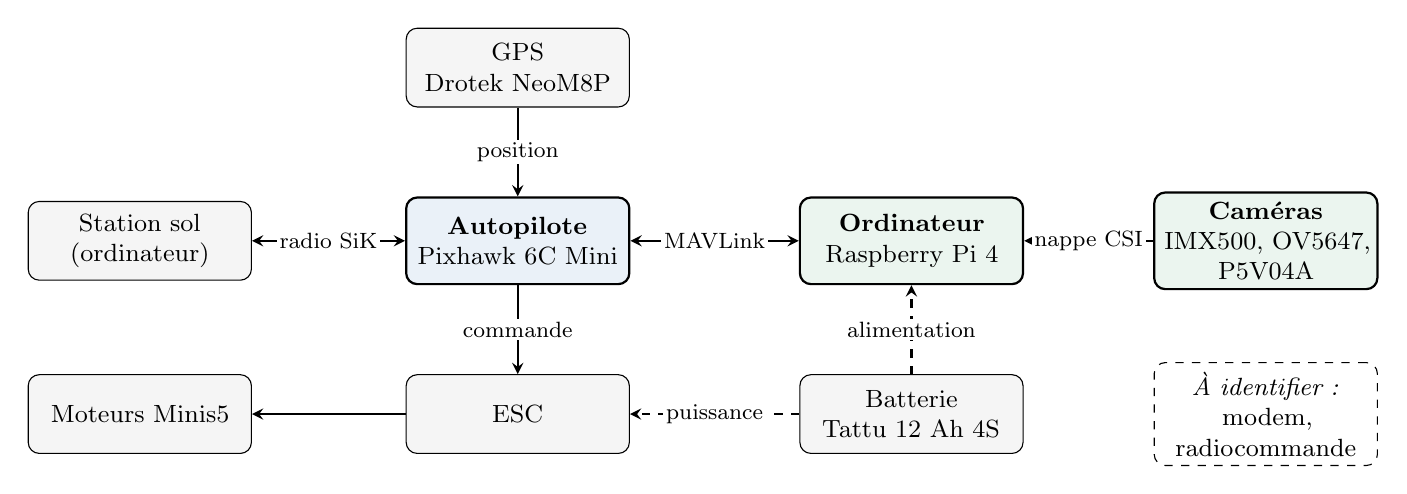
\begin{tikzpicture}[font=\small,
  bloc/.style={draw, rounded corners, fill=gray!8, align=center, text width=2.6cm, minimum height=1cm},
  bord/.style={draw, rounded corners, thick, fill=lotA!10, align=center, text width=2.6cm, minimum height=1.1cm},
  vis/.style={draw, rounded corners, thick, fill=lotB!10, align=center, text width=2.6cm, minimum height=1.1cm},
  lien/.style={->, >=stealth, thick},
  et/.style={font=\footnotesize, fill=white, inner sep=1pt}]
  \node[bord] (px) at (0,0) {\textbf{Autopilote}\\ Pixhawk 6C Mini};
  \node[vis] (rpi) at (5,0) {\textbf{Ordinateur}\\ Raspberry Pi 4};
  \node[vis] (cam) at (9.5,0) {\textbf{Caméras}\\ IMX500, OV5647, P5V04A};
  \node[bloc] (gps) at (0,2.2) {GPS\\ Drotek NeoM8P};
  \node[bloc] (sol) at (-4.8,0) {Station sol\\ (ordinateur)};
  \node[bloc] (esc) at (0,-2.2) {ESC};
  \node[bloc] (mot) at (-4.8,-2.2) {Moteurs Minis5};
  \node[bloc] (bat) at (5,-2.2) {Batterie\\ Tattu 12 Ah 4S};
  \node[draw, dashed, rounded corners, align=center, text width=2.6cm, minimum height=1cm] (man) at (9.5,-2.2) {\textit{À identifier :}\\ modem, radiocommande};
  \draw[lien] (gps) -- node[et]{position} (px);
  \draw[<->, >=stealth, thick] (sol) -- node[et]{radio SiK} (px);
  \draw[<->, >=stealth, thick] (px) -- node[et]{MAVLink} (rpi);
  \draw[lien] (cam) -- node[et]{nappe CSI} (rpi);
  \draw[lien] (px) -- node[et]{commande} (esc);
  \draw[lien] (esc) -- (mot);
  \draw[lien, dashed] (bat) -- node[et]{puissance} (esc);
  \draw[lien, dashed] (bat) -- node[et]{alimentation} (rpi);
\end{tikzpicture}}
\caption{Schéma d'assemblage provisoire des composants (traits pleins : données ; pointillés : énergie)}
\label{fig:architecture}
\end{figure}

\paragraph{Logiciels.} ArduPilot, QGroundControl, MAVLink, Python et YOLO, cités par la fiche du sujet ; GitHub pour le code.

\paragraph{Environnements.} Développement sur les ordinateurs de l'équipe et en salle de projet à l'école ; code partagé sur GitHub. Essais sur l'eau dans un lieu à définir ; la portée de la radio reste à vérifier.

\paragraph{Données d'entrée.} Le Cerema fournit le travail 2025 sur clé USB ; les scénarios de mission et les contraintes de fonctionnement restent à préciser avec le client.

\paragraph{Bibliographie.} Les ressources fournies par le client et celles identifiées par l'équipe figurent en section~\ref{sec:bibliographie}.
\\

\section{Organisation}
\label{sec:organisation}

% ---------------------------------------------------------------------------
\subsection{Présentation de l'équipe}
\label{sec:equipe}

L'équipe compte six élèves de trois filières : MCE (Mathematical and Computational Engineering), OPE (Observation and Perception of the Environment) et SEH (Embedded and Heterogeneous Systems). Elle se répartit en deux groupes de trois, vision embarquée et intégration du bateau ; cette répartition pourra évoluer (tableau~\ref{tab:equipe}).

\begin{table}[H]
\centering
\small
\caption{Membres de l'équipe : filière, compétences et rôles}
\label{tab:equipe}
\begin{tabularx}{\textwidth}{@{}p{2.8cm}p{1cm}Lp{2.9cm}p{2cm}@{}}
\toprule
\textbf{Membre} & \textbf{Filière} & \textbf{Compétences} & \textbf{Rôle organisationnel} & \textbf{Rôle technique} \\
\midrule
Guillaume Leroy & MCE & Programmation en Python, traitement du signal ; centres d'intérêt : mathématiques, IA & Responsable projet & Vision embarquée \\
\addlinespace
Reda El Mekkaoui & MCE & Machine learning, vision par ordinateur ; centres d'intérêt : IA, systèmes embarqués & Responsable communication client & Vision embarquée \\
\addlinespace
Adam-Sabri Hlaoua & MCE & Traitement d'image, machine learning, programmation en Python & Responsable comptes rendus & Vision embarquée \\
\addlinespace
Ewen Gourmelen & OPE & Robotique et automatisme, physique des capteurs, conception mécanique et électronique & Responsable matériel & Intégration du bateau \\
\addlinespace
Rana Brini & OPE & Traitement du signal, de l'image et de l'information, architecture et fonctionnement des capteurs physiques, machine learning appliqué & Responsable matériel & Intégration du bateau \\
\addlinespace
Selma Ben-Abdelkader & SEH & Conception de circuits numériques, deep learning, intelligence artificielle & Responsable livrables & Intégration du bateau \\
\bottomrule
\end{tabularx}
\end{table}

\paragraph{Acquis et formations nécessaires.}
L'équipe connaît déjà Arduino, les réseaux de neurones et la vision par ordinateur. Elle doit se former à ArduPilot et QGroundControl, à MAVLink, à l'électronique du bateau, au Raspberry Pi avec la caméra IMX500 et à YOLO embarqué. Elle s'appuiera sur de la documentation en ligne, l'espace CERAE de l'IMT Atlantique et des outils d'IA, et sollicitera les tuteurs en cas de blocage.
\\
% ---------------------------------------------------------------------------
\subsection{Parties prenantes et ressources externes}

\begin{table}[H]
\centering
\small
\caption{Parties prenantes et ressources externes}
\label{tab:parties-prenantes}
\begin{tabularx}{\textwidth}{@{}p{2.7cm}p{2.3cm}Lp{5.2cm}@{}}
\toprule
\textbf{Nom} & \textbf{Organisme} & \textbf{Rôle} & \textbf{Contact} \\
\midrule
Antoine Douchin & Cerema & Client et tuteur entreprise (drones, traitement de données) & antoine.douchin@cerema.fr \\
Matthieu Arzel & IMT Atlantique & Tuteur école (gestion de projet, systèmes embarqués) & matthieu.arzel@imt-atlantique.fr \\
Charlotte Langlais & IMT Atlantique & Responsable de l'UE & charlotte.langlais@imt-atlantique.fr \\
Lucia Bergantin & IMT Atlantique & Experte technique (vision embarquée, modélisation 3D) & lucia.bergantin@imt-atlantique.fr \\
Groupe 11 (PCE 2025) & IMT Atlantique & Retour d'expérience sur le projet 2025 & par mail \\
\bottomrule
\end{tabularx}
\end{table}

% ---------------------------------------------------------------------------
\subsection{Structure du projet}
\label{sec:structure}

Le projet est découpé en quatre lots (figure~\ref{fig:lots}). Les volumes horaires sont des estimations, inspirées du projet 2025.

\begin{figure}[H]
\centering
\resizebox{\textwidth}{!}{%
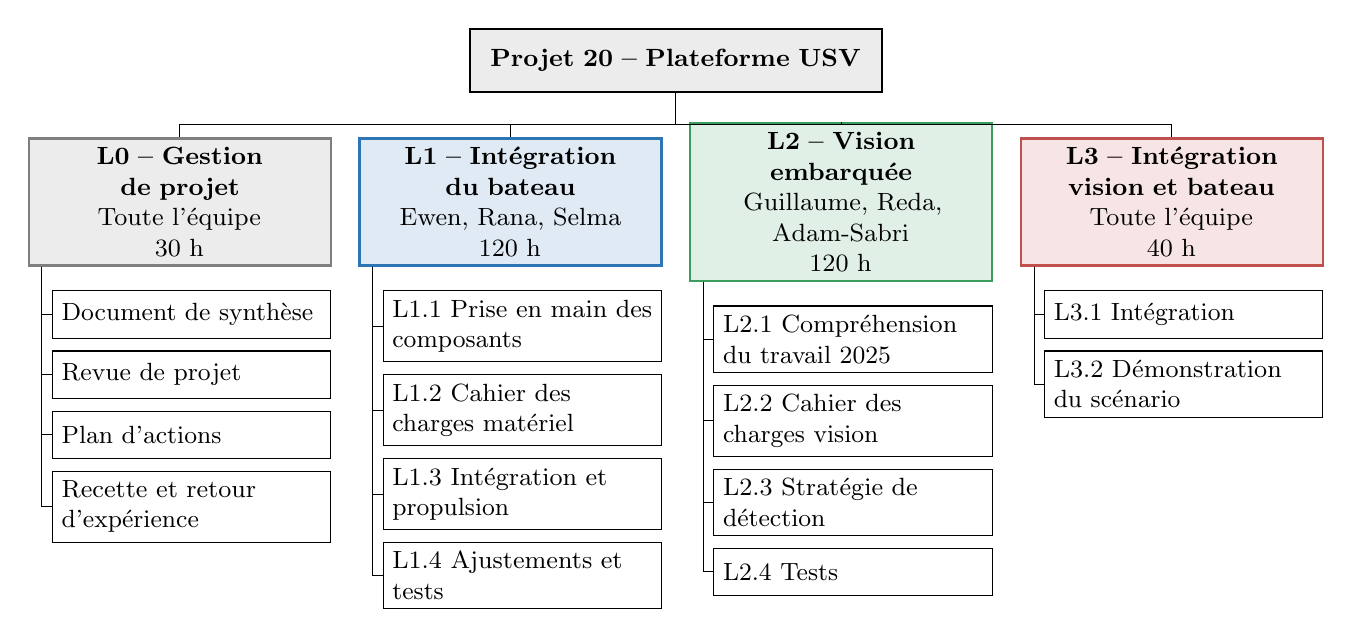
\begin{tikzpicture}[font=\small,
  racine/.style={draw, thick, fill=gray!15, align=center, text width=5cm, minimum height=0.8cm},
  lot/.style={draw, thick, align=center, text width=3.6cm, minimum height=1.5cm},
  sl/.style={draw, align=left, text width=3.3cm, minimum height=0.6cm}]
  \node[racine] (p) at (6.3,1.8) {\textbf{Projet 20 -- Plateforme USV}};
  \node[lot, fill=lotD!15, draw=lotD] (l0) at (0,0) {\textbf{L0 -- Gestion de projet}\\ Toute l'équipe\\ 30 h};
  \node[lot, fill=lotA!15, draw=lotA] (l1) at (4.2,0) {\textbf{L1 -- Intégration du bateau}\\ Ewen, Rana, Selma\\ 120 h};
  \node[lot, fill=lotB!15, draw=lotB] (l2) at (8.4,0) {\textbf{L2 -- Vision embarquée}\\ Guillaume, Reda, Adam-Sabri\\ 120 h};
  \node[lot, fill=lotC!15, draw=lotC] (l3) at (12.6,0) {\textbf{L3 -- Intégration vision et bateau}\\ Toute l'équipe\\ 40 h};
  \foreach \l in {l0,l1,l2,l3} \draw (p.south) -- ++(0,-0.4) -| (\l.north);
  \node[sl, below=0.3cm of l0, xshift=0.15cm] (a1) {Document de synthèse};
  \node[sl, below=0.15cm of a1] (a2) {Revue de projet};
  \node[sl, below=0.15cm of a2] (a3) {Plan d'actions};
  \node[sl, below=0.15cm of a3] (a4) {Recette et retour d'expérience};
  \node[sl, below=0.3cm of l1, xshift=0.15cm] (b1) {L1.1 Prise en main des composants};
  \node[sl, below=0.15cm of b1] (b2) {L1.2 Cahier des charges matériel};
  \node[sl, below=0.15cm of b2] (b3) {L1.3 Intégration et propulsion};
  \node[sl, below=0.15cm of b3] (b4) {L1.4 Ajustements et tests};
  \node[sl, below=0.3cm of l2, xshift=0.15cm] (c1) {L2.1 Compréhension du travail 2025};
  \node[sl, below=0.15cm of c1] (c2) {L2.2 Cahier des charges vision};
  \node[sl, below=0.15cm of c2] (c3) {L2.3 Stratégie de détection};
  \node[sl, below=0.15cm of c3] (c4) {L2.4 Tests};
  \node[sl, below=0.3cm of l3, xshift=0.15cm] (d1) {L3.1 Intégration};
  \node[sl, below=0.15cm of d1] (d2) {L3.2 Démonstration du scénario};
  \foreach \l/\s in {l0/a1,l0/a2,l0/a3,l0/a4,l1/b1,l1/b2,l1/b3,l1/b4,l2/c1,l2/c2,l2/c3,l2/c4,l3/d1,l3/d2}
    \draw ([xshift=-1.75cm]\l.south) |- (\s.west);
\end{tikzpicture}}
\caption{Organigramme des lots, avec responsables et volume horaire estimé}
\label{fig:lots}
\end{figure}

% ---------------------------------------------------------------------------
\subsection{Planification}

Le diagramme de Gantt (figure~\ref{fig:gantt}) place les lots et les jalons dans le temps, d'après le calendrier de l'UE (tableau~\ref{tab:jalons}). Les réunions client, toutes les deux semaines à partir du jeudi 15/10/2026, marquent les itérations.

\begin{figure}[H]
\centering
\begin{ganttchart}[
    x unit=0.92cm, y unit chart=0.55cm, y unit title=0.55cm,
    vgrid={*1{gray!25, dotted}}, hgrid={*1{gray!15}},
    canvas/.append style={draw=gray!50},
    title/.append style={draw=gray!50, fill=gray!10},
    title label font=\small\bfseries, bar label font=\small,
    group label font=\small\bfseries, milestone label font=\small\itshape,
    bar height=.6, group height=.45, group top shift=.28,
    group left shift=0, group right shift=0, group peaks height=0, group peaks width=0,
    milestone height=.6,
  ]{1}{12}
  \gantttitle{Sept.}{1} \gantttitle{Octobre}{4} \gantttitle{Novembre}{4} \gantttitle{Décembre}{3} \\
  \gantttitle[title label font=\footnotesize]{28/09}{1}
  \gantttitle[title label font=\footnotesize]{05/10}{1}
  \gantttitle[title label font=\footnotesize]{12/10}{1}
  \gantttitle[title label font=\footnotesize]{19/10}{1}
  \gantttitle[title label font=\footnotesize]{26/10}{1}
  \gantttitle[title label font=\footnotesize]{02/11}{1}
  \gantttitle[title label font=\footnotesize]{09/11}{1}
  \gantttitle[title label font=\footnotesize]{16/11}{1}
  \gantttitle[title label font=\footnotesize]{23/11}{1}
  \gantttitle[title label font=\footnotesize]{30/11}{1}
  \gantttitle[title label font=\footnotesize]{07/12}{1}
  \gantttitle[title label font=\footnotesize]{14/12}{1} \\
  \ganttgroup[group/.append style={fill=lotD, draw=lotD}]{L0 -- Gestion de projet}{1}{12} \\
  \ganttgroup[group/.append style={fill=lotA, draw=lotA}]{L1 -- Intégration du bateau}{1}{10} \\
  \ganttbar[bar/.append style={fill=lotA!30, draw=lotA}, name=b11]{Prise en main des composants}{1}{3} \\
  \ganttbar[bar/.append style={fill=lotA!30, draw=lotA}, name=b12]{Cahier des charges matériel}{3}{4} \\
  \ganttbar[bar/.append style={fill=lotA!30, draw=lotA}, name=b13]{Intégration et propulsion}{4}{8} \\
  \ganttbar[bar/.append style={fill=lotA!30, draw=lotA}, name=b14]{Ajustements et tests}{8}{10} \\
  \ganttgroup[group/.append style={fill=lotB, draw=lotB}]{L2 -- Vision embarquée}{1}{9} \\
  \ganttbar[bar/.append style={fill=lotB!30, draw=lotB}, name=b21]{Compréhension du travail 2025}{1}{2} \\
  \ganttbar[bar/.append style={fill=lotB!30, draw=lotB}, name=b22]{Cahier des charges vision}{3}{4} \\
  \ganttbar[bar/.append style={fill=lotB!30, draw=lotB}, name=b23]{Stratégie de détection}{4}{7} \\
  \ganttbar[bar/.append style={fill=lotB!30, draw=lotB}, name=b24]{Tests}{7}{9} \\
  \ganttgroup[group/.append style={fill=lotC, draw=lotC}]{L3 -- Intégration vision et bateau}{10}{12} \\
  \ganttbar[bar/.append style={fill=lotC!30, draw=lotC}, name=b31]{Intégration}{10}{11} \\
  \ganttbar[bar/.append style={fill=lotC!30, draw=lotC}, name=b32]{Démonstration du scénario}{11}{12} \\
  \ganttgroup[group/.append style={draw=none, fill=none}]{Jalons}{1}{12} \\
  \ganttmilestone[milestone left shift=.3, milestone right shift=-.3, milestone/.append style={fill=black}]{J1 -- Document de synthèse}{1} \\
  \ganttmilestone[milestone left shift=.3, milestone right shift=-.3, milestone/.append style={fill=black}]{J2 -- Prise en main du bateau}{3} \\
  \ganttmilestone[milestone left shift=.3, milestone right shift=-.3, milestone/.append style={fill=black}]{J3 -- Revue de projet}{4} \\
  \ganttmilestone[milestone left shift=.3, milestone right shift=-.3, milestone/.append style={fill=black}]{J4 -- Cahiers des charges précis}{4} \\
  \ganttmilestone[milestone left shift=.3, milestone right shift=-.3, milestone/.append style={fill=black}]{J5 -- Plan d'actions}{6} \\
  \ganttmilestone[milestone left shift=.3, milestone right shift=-.3, milestone/.append style={fill=black}]{J6 -- Bateau suivant un cap}{8} \\
  \ganttmilestone[milestone left shift=.3, milestone right shift=-.3, milestone/.append style={fill=black}]{J7 -- Vision fonctionnelle}{9} \\
  \ganttmilestone[milestone left shift=.3, milestone right shift=-.3, milestone/.append style={fill=black}]{J8 -- Recette}{12} \\
  \ganttmilestone[milestone left shift=.3, milestone right shift=-.3, milestone/.append style={fill=gray!60, draw=gray!80}]{Réunions client}{3}
    \ganttmilestone[milestone left shift=.3, milestone right shift=-.3, milestone/.append style={fill=gray!60, draw=gray!80}]{}{5}
    \ganttmilestone[milestone left shift=.3, milestone right shift=-.3, milestone/.append style={fill=gray!60, draw=gray!80}]{}{7}
    \ganttmilestone[milestone left shift=.3, milestone right shift=-.3, milestone/.append style={fill=gray!60, draw=gray!80}]{}{9}
    \ganttmilestone[milestone left shift=.3, milestone right shift=-.3, milestone/.append style={fill=gray!60, draw=gray!80}]{}{11}
  % Dépendances fin -> début (flèches tracées en TikZ, voir \ganttdep dans le préambule)
  \ganttdep{b11}{b12} \ganttdep{b12}{b13} \ganttdep{b13}{b14}
  \ganttdep{b21}{b22} \ganttdep{b22}{b23} \ganttdep{b23}{b24}
  \ganttdep[0.825cm]{b14}{b31} \ganttdep[0.825cm]{b24}{b31} \ganttdep{b31}{b32}
\end{ganttchart}
\caption{Diagramme de Gantt. Colonnes : semaines, désignées par la date du lundi. Flèches : dépendances entre tâches (une tâche commence quand la précédente est terminée). Losanges noirs : jalons (tableau~\ref{tab:jalons}) ; losanges gris : réunions client prévues.}
\label{fig:gantt}
\end{figure}

\begin{table}[H]
\centering
\small
\caption{Jalons}
\label{tab:jalons}
\begin{tabularx}{\textwidth}{@{}p{0.7cm}p{4cm}Lp{1.1cm}p{1.9cm}@{}}
\toprule
\textbf{Id.} & \textbf{Jalon} & \textbf{Critère} & \textbf{Lot} & \textbf{Date} \\
\midrule
J1 & Document de synthèse & Envoyé au client et au tuteur & L0 & 02/10/2026 \\
J2 & Prise en main du bateau & Moteurs commandés, bateau piloté à distance & L1 & 16/10/2026 \\
J3 & Revue de projet & Déposée sur Moodle & L0 & 19/10/2026 \\
J4 & Cahiers des charges précis & Validés par le Cerema & L1, L2 & 23/10/2026 \\
J5 & Plan d'actions & Déposé sur Moodle & L0 & 05/11/2026 \\
J6 & Bateau suivant un cap & Suivi de cap, arrêt & L1 & 20/11/2026 \\
J7 & Vision fonctionnelle & Détection testée, y compris par mauvais temps & L2 & 27/11/2026 \\
J8 & Recette & Scénario complet démontré au client et au tuteur & L3, L0 & 18/12/2026 \\
\bottomrule
\end{tabularx}
\end{table}

\begin{table}[H]
\centering
\small
\caption{Livrables}
\label{tab:livrables}
\begin{tabularx}{\textwidth}{@{}Lp{2.3cm}p{3.4cm}p{2.3cm}@{}}
\toprule
\textbf{Livrable} & \textbf{Type} & \textbf{Destinataire} & \textbf{Échéance} \\
\midrule
Document de synthèse & Organisationnel & Client et école & 02/10/2026 \\
Revue de projet & Organisationnel & École & 19/10/2026 \\
Plan d'actions & Organisationnel & École & 05/11/2026 \\
Cahiers des charges précis & Technique & Client & 23/10/2026 \\
Code (dépôt GitHub) & Technique & Client & En continu \\
Documentation technique et procédures d'utilisation & Technique & Client & 18/12/2026 \\
Recette du projet & Organisationnel & Client et tuteur école & 18/12/2026 \\
Retour d'expérience & Organisationnel & École & Décembre 2026 \\
Posters et forum & Organisationnel & École & Janvier 2027 \\
\bottomrule
\end{tabularx}
\end{table}

% ---------------------------------------------------------------------------
\subsection{Communication et partage}

Reda El Mekkaoui est l'interlocuteur du client ; Adam-Sabri Hlaoua rédige les comptes rendus, partagés avec le client et le tuteur après chaque réunion (tableau~\ref{tab:communication}).

\begin{table}[H]
\centering
\small
\caption{Moyens de communication et de partage}
\label{tab:communication}
\begin{tabularx}{\textwidth}{@{}p{3cm}Lp{3.2cm}L@{}}
\toprule
\textbf{Avec qui} & \textbf{Moyen} & \textbf{Fréquence} & \textbf{Outils} \\
\midrule
Équipe & Point d'avancement en présentiel & Chaque semaine & WhatsApp \\
Tuteur école & Réunion à l'école & Toutes les deux semaines & E-mail \\
Client (Cerema) & Réunion à l'école & Toutes les deux semaines & E-mail \\
Documents et code & Partage avec le client et le tuteur & En continu & GitHub, espace de partage IMT \\
\bottomrule
\end{tabularx}
\end{table}

% ---------------------------------------------------------------------------
\subsection{Analyse des risques}
\label{sec:risques}

Le tableau~\ref{tab:risques} présente l'analyse initiale des risques ; elle sera mise à jour à mi-projet et en fin de projet. Pour chaque risque, la probabilité (P) et la gravité (G) sont notées de 1 à 3 ; la criticité est leur produit, de 1--2 (faible, vert) à 6--9 (élevée, rouge).

\begin{table}[H]
\centering
\small
\setlength{\tabcolsep}{4pt}
\caption{Analyse initiale des risques}
\label{tab:risques}
\begin{tabularx}{\textwidth}{@{}>{\raggedright\arraybackslash}p{2.9cm}cc>{\centering\arraybackslash}p{1.7cm}LLp{1.9cm}@{}}
\toprule
\textbf{Risque} & \textbf{P} & \textbf{G} & \textbf{Criticité} & \textbf{Prévention} & \textbf{Correction} & \textbf{Responsable} \\
\midrule
Manque de temps & 2 & 2 & \cellcolor{critiqueMed}4 -- Moyenne & Planifier avec marge ; fixer des jalons intermédiaires stricts & Prioriser la navigation puis la détection ; identification en option & Guillaume \\
\addlinespace
Composants manquants ou inadaptés (modem, radio) & 2 & 2 & \cellcolor{critiqueMed}4 -- Moyenne & Inventorier et tester le matériel dès la prise en main & Signaler immédiatement au Cerema ; basculer sur des modules de rechange & Ewen, Rana \\
\addlinespace
Prise en main longue des outils (ArduPilot, MAVLink) & 2 & 2 & \cellcolor{critiqueMed}4 -- Moyenne & Se former dès le début avec les tutoriels et documentations officielles & Solliciter les tuteurs ; s'appuyer sur des exemples validés & Chaque groupe \\
\addlinespace
Pas de jeu de données adapté à la détection & 2 & 2 & \cellcolor{critiqueMed}4 -- Moyenne & Réutiliser et vérifier l'exhaustivité du jeu de données 2025 & Collecter rapidement des images réelles ; augmentation de données & Groupe vision \\
\addlinespace
Rupture de la coque, voie d'eau, chavirage & 1 & 3 & \cellcolor{critiqueMed}3 -- Moyenne & Premiers essais en eau calme ; caisson électronique étanche testé à vide & Procédure d'arrêt d'urgence ; flottaison et récupération immédiate & Groupe intégration \\
\addlinespace
Optique abîmée par l'eau de mer ou la pluie & 2 & 2 & \cellcolor{critiqueMed}4 -- Moyenne & Boîtier étanche avec traitement hydrophobe pour l'objectif & Nettoyage ou remplacement de l'optique ; modèle entraîné sur images dégradées & Groupe vision \\
\addlinespace
Incident sur batterie lithium (court-circuit, feu) & 1 & 3 & \cellcolor{critiqueMed}3 -- Moyenne & Charge sous surveillance stricte ; stockage en sac LiPo ignifugé & Extincteur adapté à proximité ; coupe-circuit général d'urgence & Ewen, Rana \\
\addlinespace
Surconsommation du Raspberry Pi & 2 & 1 & \cellcolor{critiqueLow}2 -- Faible & Optimiser les algorithmes ; choisir un modèle léger & Détection en basse résolution ou cadence de traitement réduite & Groupe vision \\
\addlinespace
Perte de liaison radio ou télémétrie en mer & 2 & 3 & \cellcolor{critiqueHigh}\textbf{6} -- Élevée & Vérifier la portée radio à quai ; antennes orientées et dégagées & Failsafe ArduPilot automatique (retour au point de départ) et arrêt des propulseurs & Groupe intégration \\
\addlinespace
Perte du signal GPS ou dérive du compas & 2 & 3 & \cellcolor{critiqueHigh}\textbf{6} -- Élevée & Étalonner le compas loin des masses métalliques ; vérifier le HDOP avant départ & Passage immédiat en pilotage manuel par radiocommande & Groupe intégration \\
\addlinespace
Conditions météo défavorables (vent, clapot) & 2 & 2 & \cellcolor{critiqueMed}4 -- Moyenne & Consulter les bulletins météo côtiers avant chaque essai & Reporter les essais en mer ; simulation et travail logiciel à quai & Toute l'équipe \\
\bottomrule
\end{tabularx}
\end{table}

\section{Validation du projet}
\label{sec:validation-projet}

Le tableau~\ref{tab:validation} reprend, dans le même ordre, chaque fonction du tableau~\ref{tab:fonctions} avec son niveau, et précise comment elle sera validée, par qui et à quel jalon. Les seuils restent à valider avec le Cerema. Les trois dernières lignes portent sur le projet dans son ensemble.

\begin{table}[H]
\centering
\small
\caption{Critères de validation des fonctions du tableau~\ref{tab:fonctions} et du projet}
\label{tab:validation}
\begin{tabularx}{\textwidth}{@{}>{\raggedright\arraybackslash}p{3.2cm}Lp{3.2cm}p{2.2cm}p{0.9cm}@{}}
\toprule
\textbf{Fonction} & \textbf{Méthode} & \textbf{Seuil} & \textbf{Responsable} & \textbf{Jalon} \\
\midrule
FP1 -- Pilotage manuel à distance & Essai sur l'eau & Réponse < 1 s & Groupe intégration & J2 \\
FP2 -- Détection des navires & Tests sur images réelles et dégradées (pluie, roulis, mouvement) & Taux $\geq$ 90~\% ; au moins 1 image analysée toutes les 5 s & Groupe vision & J7 \\
FP3 -- Transmission de l'état de la mission & Test de communication entre la station sol et le bateau & Au moins 1 mise à jour par minute & Groupe intégration & J6 \\
FP4 -- Alerte à l'opérateur & Démonstration & $\leq$ 5 s après la détection & Groupe vision & J8 \\
FP5 -- Suivi autonome d'un cap et d'une trace GPS & Essai sur l'eau & Écart $\leq$ 5 m à chaque point de passage & Groupe intégration & J6 \\
FS1 -- Identification des navires & Tests sur images de navires connus, si la fonction est réalisée & À définir avec le Cerema & Groupe vision & J8 \\
FS2 -- Approche du navire suspect & Essai sur l'eau, si la fonction est réalisée & Écart $\leq$ 5 m par rapport à la trajectoire calculée & Toute l'équipe & J8 \\
FC1 -- Matériel mis à disposition & Revue du matériel utilisé & Matériel du tableau~\ref{tab:materiel} & Groupe intégration & J4 \\
FC2 -- Protocole MAVLink & Vérification des échanges entre l'ordinateur compagnon et l'autopilote & MAVLink & Groupe intégration & J8 \\
FC3 -- Consommation énergétique & Essai d'endurance sur l'eau & Au moins 1 h d'essai en continu & Groupe intégration & J8 \\
FC4 -- Sécurité & Coupure volontaire de la liaison & Arrêt des moteurs & Groupe intégration & J2 \\
\midrule
Cahier des charges & Revue avec le Cerema & Validé par le client & Toute l'équipe & J4 \\
Scénario complet (FP1 à FP5) & Démonstration au client et au tuteur & Patrouille, détection, alerte, reprise en main & Toute l'équipe & J8 \\
Livrables & Dépôt sur Moodle et GitHub & Dans les délais & Selma & J1 à J8 \\
\bottomrule
\end{tabularx}
\end{table}

\section{Conclusion}
\label{sec:conclusion}

Cette première phase a fixé la problématique, les objectifs, le périmètre et l'organisation en deux groupes. En phase 2 (Production), chaque groupe commence par la prise en main : les composants du bateau d'un côté, le travail 2025 en vision de l'autre. Les prochaines étapes clés sont la revue de projet (19/10), les cahiers des charges précis (23/10), puis le bateau suivant un cap et la vision fonctionnelle fin novembre, avant la recette du 18/12.



\section{Références bibliographiques}
\label{sec:bibliographie}

\paragraph{Ressources fournies par le client.}
\begin{itemize}
  \item Cerema, fiche du sujet numéro 20, « Intégration d'une plateforme USV et d'une chaîne de détection temps réel assistée par intelligence artificielle pour l'aide à la navigation autonome », PCE S7, IMT Atlantique, 2026-2027.
  \item Groupe 11, « Conception d'un micro drone de surface », rapport de recette finale, PCE S7 2025-2026, IMT Atlantique, 15/12/2025.
  \item Groupe 11, document de synthèse du projet « Conception d'un micro drone de surface », PCE S7 2025-2026, 02/10/2025.
  \item Travaux du projet 2025 (code, données), clé USB remise par le Cerema, septembre 2026.
  \item A. Douchin (Cerema), e-mail « Projet commande entreprise USV-IA », 25/09/2026.
  \item Réunion avec A. Douchin (Cerema) et M. Arzel (IMT Atlantique), IMT Atlantique, 02/10/2026.
\end{itemize}

\paragraph{Ressources identifiées par l'équipe.}
\begin{itemize}
  \item Documentation ArduPilot Rover : \url{https://ardupilot.org/rover/}
  \item Documentation MAVLink : \url{https://mavlink.io}
  \item Documentation QGroundControl : \url{https://docs.qgroundcontrol.com}
  \item Documentation Holybro (Pixhawk) : \url{https://docs.holybro.com}
  \item Documentation Raspberry Pi, caméra IA : \url{https://www.raspberrypi.com/documentation/accessories/ai-camera.html}
  \item Ultralytics, guide YOLO sur Raspberry Pi : \url{https://docs.ultralytics.com/fr/guides/raspberry-pi/}
  \item Modèle de dépôt GitHub proposé par le Cerema : \url{https://github.com/cnigfr/cnig-template}
\end{itemize}


%--------------------------------------- DEBUT DES ANNEXES --------------------------------------
\newpage
\begin{IMTAannexes}

\IMTAannexe{Présentation faite au client}\label{sec:presentation-client}

Présentation faite au Cerema lors de la réunion de lancement.

\medskip
\noindent
\foreach \p in {1,...,9}{%
  \includegraphics[page=\p,width=0.49\textwidth]{presentation_client.pdf}\hfill
}

\IMTAannexe{Contrat d'équipe}\label{sec:contrat-equipe}

\subsection*{Règles de fonctionnement}
\begin{enumerate}
  \item Arriver à l'heure : 8 h, au début de chaque séance.
  \item Être présent à chaque séance et rester jusqu'à la fin ; un départ anticipé (par exemple pour le repas) se décide ensemble.
  \item Prévenir à l'avance en cas d'absence.
  \item Faire un point d'avancement chaque semaine, même sans avancée.
  \item Être joignable et répondre aux messages de l'équipe.
  \item Garder une trace écrite de tout, accessible à tous (outil envisagé : Notion).
  \item S'investir dans le projet.
\end{enumerate}


\subsection*{Trois conditions essentielles}
La ponctualité, un point d'avancement chaque semaine et une trace écrite accessible à tous.

\subsection*{Réunions et outils}
Séances de projet le lundi, le jeudi et le vendredi, à partir de 8 h. Point d'équipe chaque semaine ; réunion avec le tuteur toutes les deux semaines et avec le client toutes les deux semaines, à l'école. Outils : GitHub pour le code, espace de partage IMT pour les documents, WhatsApp dans l'équipe, e-mail avec le client et le tuteur.


%------------------------------------- -- FIN DES ANNEXES --------------------------------------
\end{IMTAannexes}

%---------------------------------------- Do not modify ----------------------------------------
\IMTAcoverpage
%------------------------------------ End of do not modify -------------------------------------

\end{document}

%***********************************************************************************************
%                                   FIN DU FICHIER D'EDITION
%***********************************************************************************************
